\section{Results}
\label{sec:results}

\subsection{2D Euler equations with a one dimensional uncertainty}
\label{sec:resultsNACA1D}
We start by quantifying the effects of an uncertain angle of attack $\phi\sim U(0.75,1.75)$ for a NACA0012 airfoil computed with different methods. The stochastic Euler equations in two dimensions are given by
\begin{align*}
\partial_t
\begin{pmatrix}
\rho \\ \rho v_1 \\ \rho v_2 \\ \rho e
\end{pmatrix}
+\partial_{x_1}
\begin{pmatrix}
\rho v_1 \\ \rho v_1^2 +p \\ \rho v_1 v_2 \\  v_1 (\rho e+p)
\end{pmatrix}
+\partial_{x_2}
\begin{pmatrix}
\rho v_2 \\ \rho v_1 v_2 \\ \rho v_2^2+p \\ v_2 (\rho e+p)
\end{pmatrix}
=\bm{0}.
\end{align*}
These equations determine the time evolution of the conserved variables $(\rho,\rho \bm v, \rho e)$, i.e. density, momentum and energy. A closure for the pressure $p$ is given by
\begin{align*}
p = (\gamma-1)\rho\left(e-\frac12(v_1^2+v_2^2)\right).
\end{align*}
Here, the heat capacity ratio $\gamma$ is chosen to be $1.4$. The spatial mesh discretizes the flow domain around the airfoil. At the airfoil boundary $\Gamma_{0}$, we use the Euler slip condition $\bm v^T\bm n = 0$, where $\bm n$ denotes the surface normal. At a sufficiently large distance away from the airfoil, we assume a far field flow with a given Mach number $Ma = 0.8$, pressure $p = 101\;325$ Pa and a temperature of $273.15$ K. Now the angle of attack $\phi$ is uniformly distributed in the interval of $[0.75,1.75]$ degrees, i.e. we choose $\phi(\xi) = 1.25 + 0.5\xi$ where $\xi\sim U(-1,1)$. As commonly done, the initial condition is equal to the far field boundary values. Consequently, the wall condition at the airfoil is violated initially and will correct the flow solution. 

The computational domain is a circle with a diameter of $40$ meters. In the center, the NACA0012 airfoil with a length of one meter is located. The spatial mesh is composed of a coarsely discretized far field and a finely resolved region around the airfoil, since we are interested in the flow solution at the airfoil. Altogether, the mesh consists of 22361 triangular elements.

\begin{figure}[h!]
\centering
	\begin{subfigure}{0.5\linewidth}
		\centering
				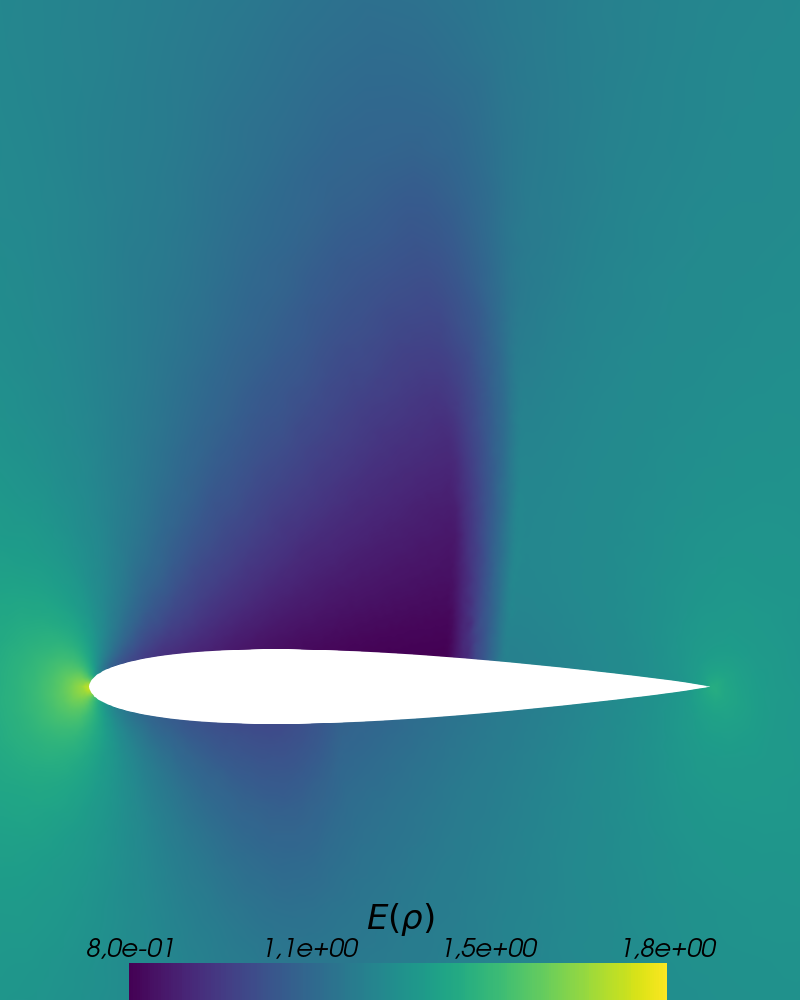
\includegraphics[scale=0.2]{figs/Euler1DPlots5/sc100_ERho.png}
		\label{fig:referenceSolutionsub1}
	\end{subfigure}%
	\begin{subfigure}{0.5\linewidth}
		\centering
				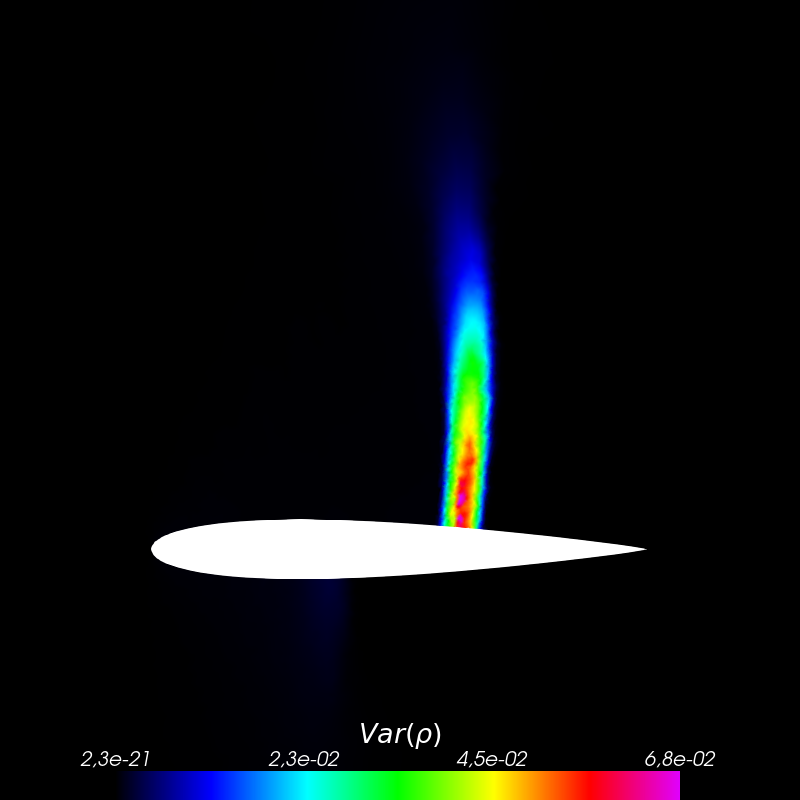
\includegraphics[scale=0.2]{figs/Euler1DPlots5/sc100_VarRho.png}
		\label{fig:referenceSolutionsub2}
	\end{subfigure}
	\caption{Reference solution E$[\rho]$ and Var$[\rho]$.}
	\label{fig:referenceSolution}
\end{figure}

The aim is to quantify the effects arising from the one-dimensional uncertainty $\xi$ and to investigate its effects on the solution with different methods. To be able to measure the quality of the obtained solutions, we compute a reference solution using stochastic-Collocation with $100$ Gauss-Legendre quadrature points, which can be found in Figure~\ref{fig:referenceSolution}. In the following, we investigate the L$^2$-error of the variance and the expectation value. The L$^2$-error of the discrete quantity $\bm e_{\Delta}=(\bm e_1,\cdots,\bm e_{N_x})^T$, where $\bm e_j$ denotes the cell average in spatial cell $j$ is denoted by
\begin{align*}
\Vert \bm e_{\Delta} \Vert_{\Delta} := \sqrt{\sum_{j=1}^{N_x} \Delta x_j \bm e_j^2}.
\end{align*}
Hence, when denoting the reference solution by $\bm u_{\Delta}$ and the moments obtained with the numerical method by $\hat{\bm u}_{\Delta}$, we investigate the relative error
\begin{align*}
\frac{\Vert \text{E}[\bm u_{\Delta}] - \text{E}[\mathcal{U}(\bm{\hat u}_{\Delta})] \Vert_{\Delta}}{\Vert \text{E}[\bm u_{\Delta}] \Vert_{\Delta}} \qquad \text{ and }\qquad \frac{\Vert \text{Var}[\bm u_{\Delta}] - \text{Var}[\mathcal{U}(\bm{\hat u}_{\Delta})] \Vert_{\Delta}}{\Vert \text{Var}[\bm u_{\Delta}] \Vert_{\Delta}}.
\end{align*}
The error is computed inside a box of one meter height and 1.1 meters length around the airfoil to prevent small fluctuations in the coarsely discretized far field from affecting the error.

The quantities of interests are now computed with the different methods. All methods in this section have been computed using five MPI threads. For more information on the chosen entropy and the resulting solution ansatz for IPM, see \ref{app:IPM2DEuler}. 

\begin{figure}[h!]
\centering
\centering
	\begin{subfigure}{0.5\linewidth}
		\centering
				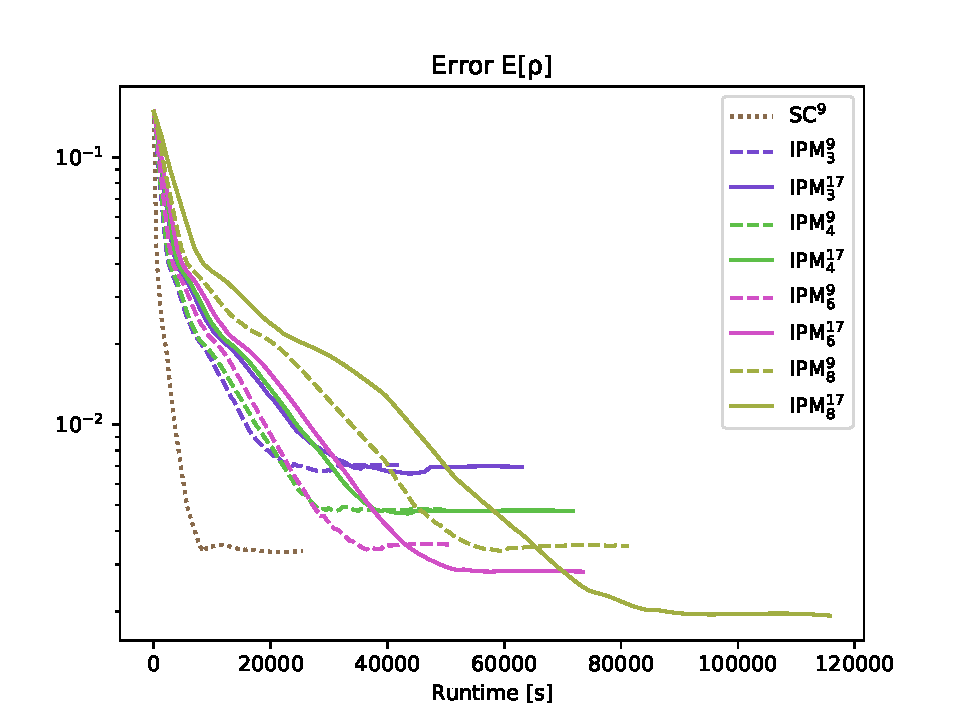
\includegraphics[scale=0.544]{figs/StudyQuadrature/L2_error_E[rho]_new.pdf}
		\caption{}
		\label{fig:ErrorDifferentQuadA}
	\end{subfigure}%
	\begin{subfigure}{0.5\linewidth}
		\centering
				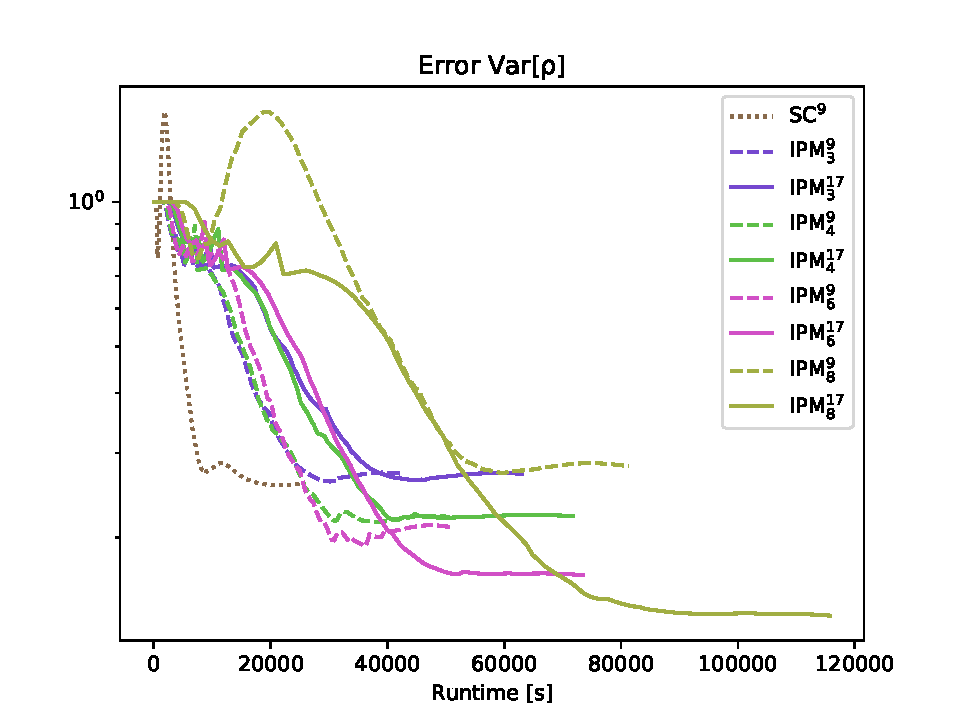
\includegraphics[scale=0.544]{figs/StudyQuadrature/L2_error_Var[rho]_new.pdf}
		\caption{}
		\label{fig:ErrorDifferentQuadB}
	\end{subfigure}
	\caption{Relative L$^2$-error with different quadrature levels for IPM in comparison with SC. The subscript denotes the moment order, the superscript denotes the number of Clenshaw-Curtis quadrature points.}
	\label{fig:ErrorDifferentQuad}
\end{figure}
\begin{figure}[h!]
\centering
	\begin{subfigure}{0.5\linewidth}
		\centering
				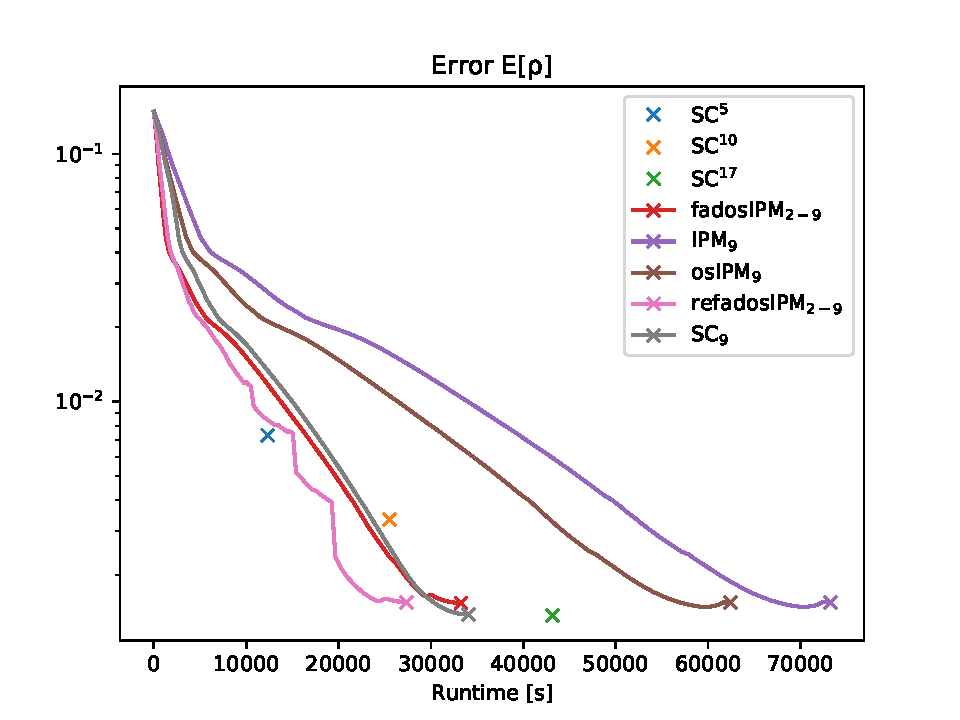
\includegraphics[scale=0.55]{figs/errorEuler/L2_error_E[rho].pdf}
		\label{fig:sub31}
		\caption{}
	\end{subfigure}%
	\begin{subfigure}{0.5\linewidth}
		\centering
				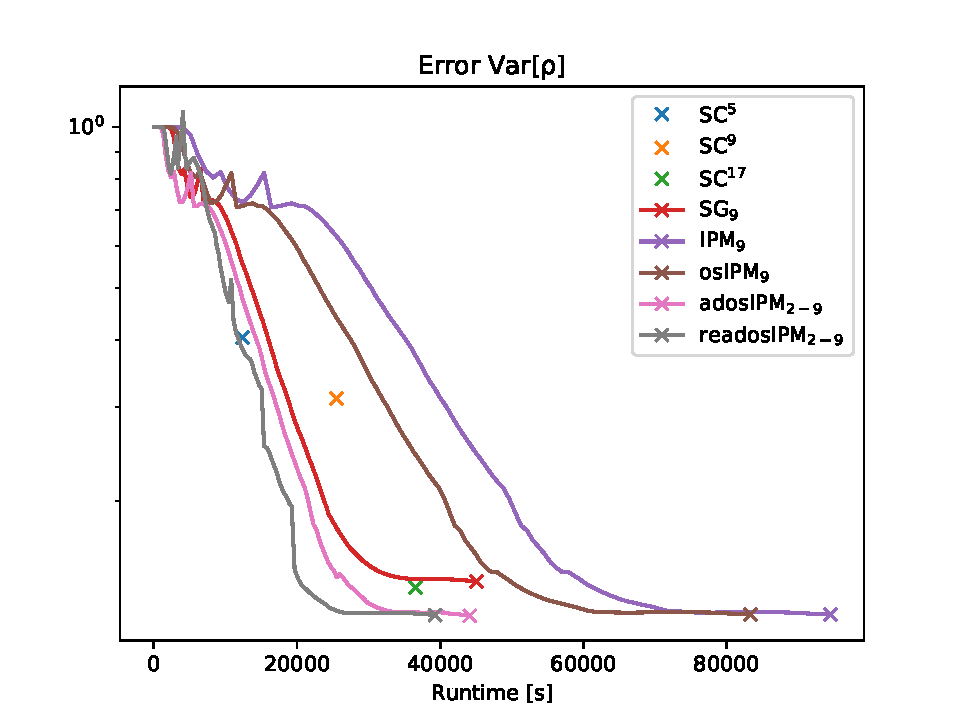
\includegraphics[scale=0.55]{figs/errorEuler/L2_error_Var[rho].pdf}
		\label{fig:sub32}
		\caption{}
	\end{subfigure}
	
	\begin{subfigure}{0.5\linewidth}
		\centering
				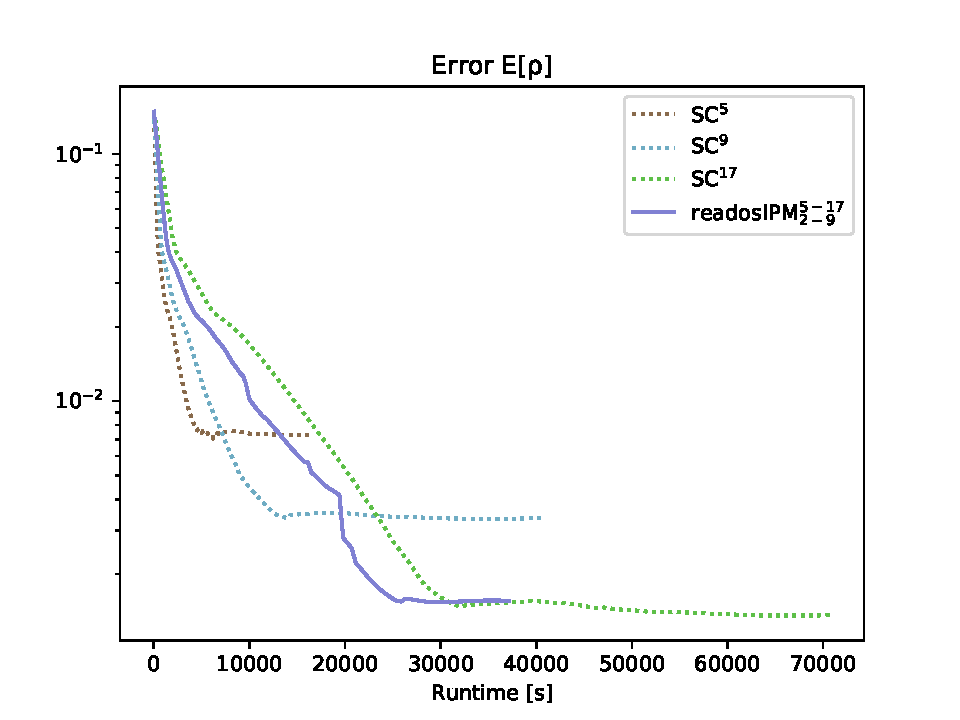
\includegraphics[scale=0.55]{figs/errorEuler/L2_error_E[rho]_sc.pdf}
		\label{fig:sub33}
		\caption{}
	\end{subfigure}%
	\begin{subfigure}{0.5\linewidth}
		\centering
				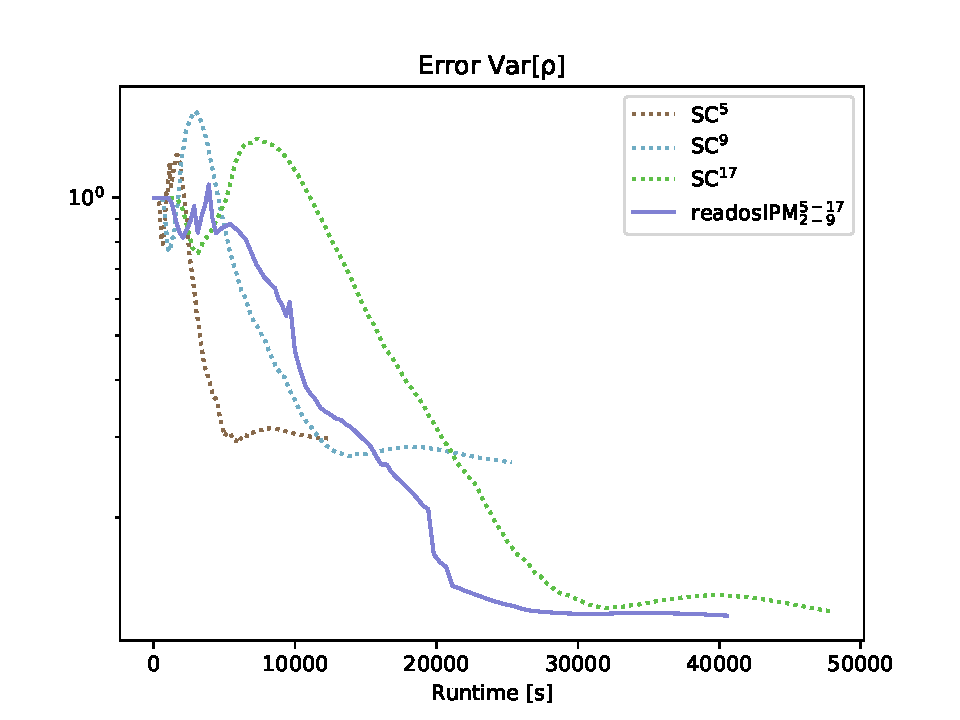
\includegraphics[scale=0.55]{figs/errorEuler/L2_error_Var[rho]_sc.pdf}
		\label{fig:sub34}
		\caption{}
	\end{subfigure}
	\caption{Comparison of the relative L$^2$-error for the density for IPM related methods (first row) and of the best performing IPM method in comparison with SC (second row). Computed with 5 MPI threads.}
	\label{fig:L2ErrorSolution}
\end{figure}
\begin{figure}[h!]
\centering
	\begin{subfigure}{0.3\linewidth}
		\centering
		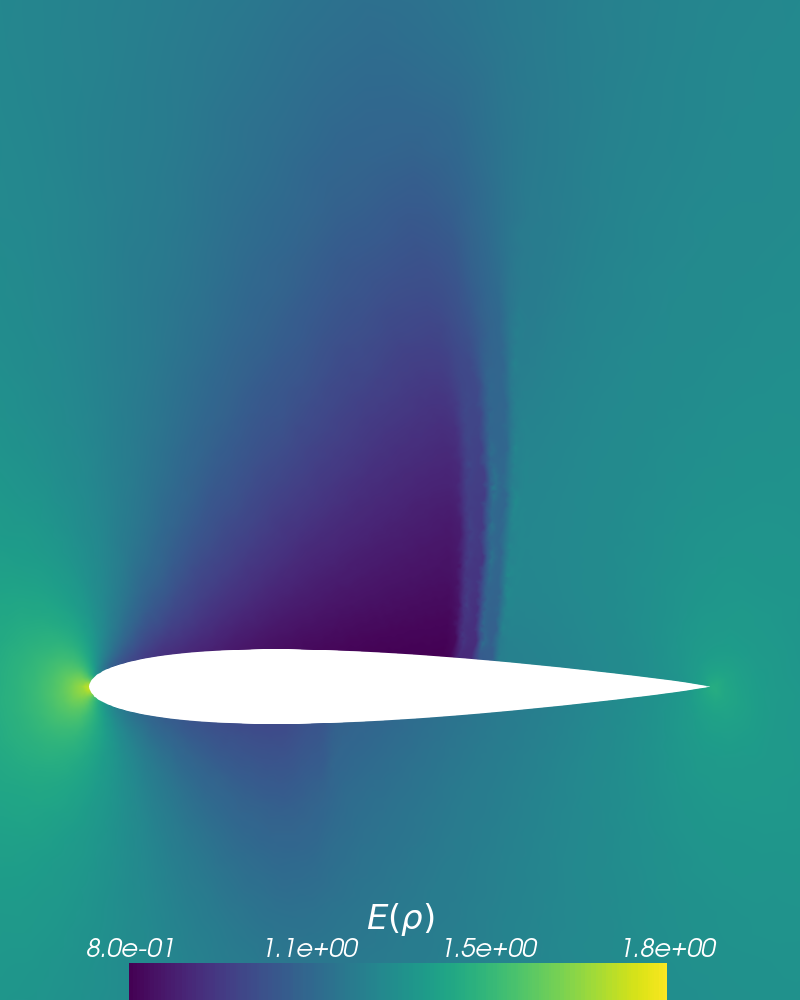
\includegraphics[scale=0.2]{figs/Euler1DPlots5/EulerSC5-2Res1e-6_ERho.png}
		\label{fig:sub1}
	\end{subfigure}%
	\hfill
	\begin{subfigure}{0.3\linewidth}
		\centering
		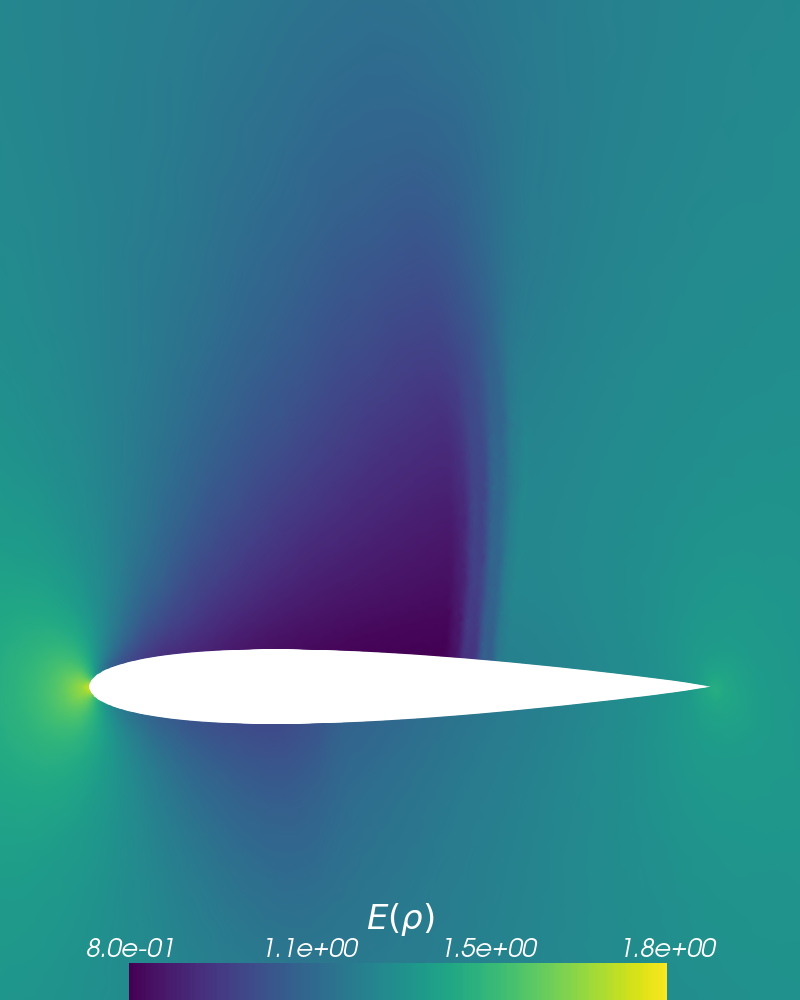
\includegraphics[scale=0.2]{figs/Euler1DPlots5/sg_4_9_ERho.png}
		\label{fig:sub2}
	\end{subfigure}%
	\hfill
	\begin{subfigure}{0.3\linewidth}
		\centering
		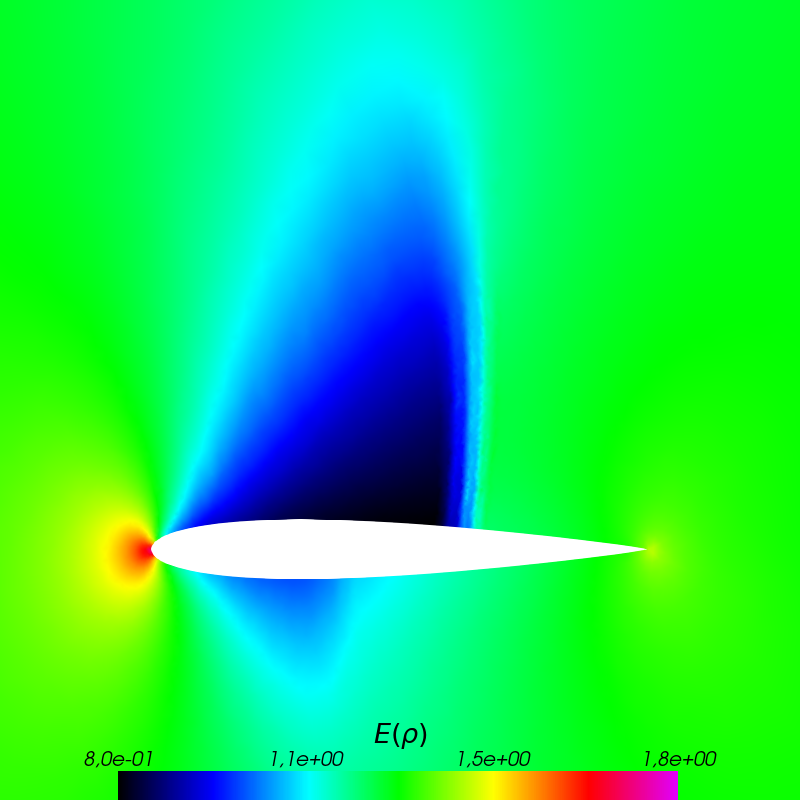
\includegraphics[scale=0.2]{figs/Euler1DPlots5/osIPM4-4_ERho.png}
		\label{fig:sub1}
	\end{subfigure}\\
	\vspace{-0.35cm}
	\begin{subfigure}{0.3\linewidth}
		\centering
		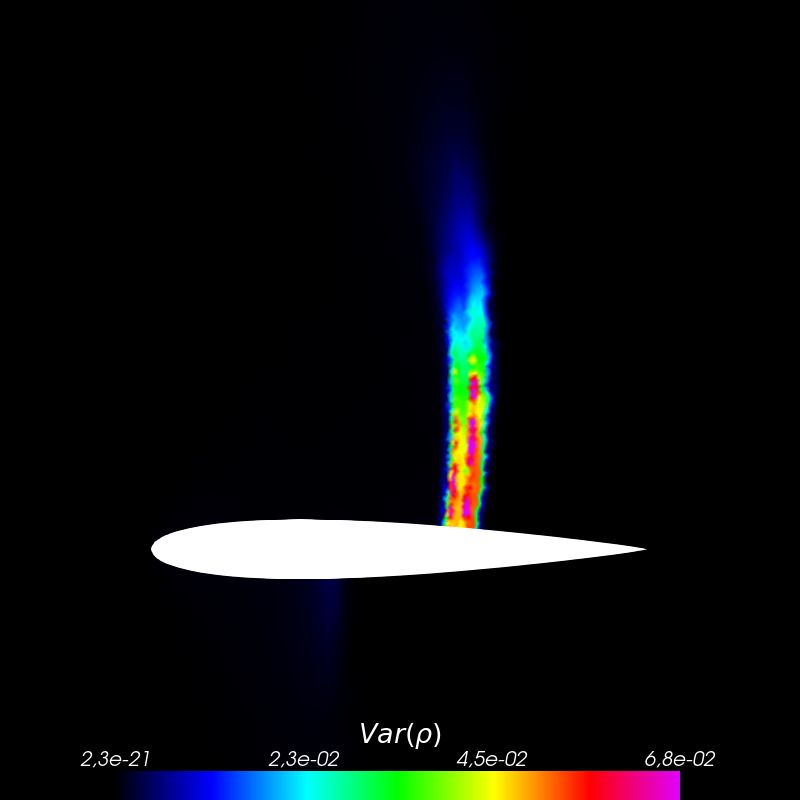
\includegraphics[scale=0.2]{figs/Euler1DPlots5/EulerSC5-2Res1e-6_VarRho.png}
		\label{fig:sub1}
	\end{subfigure}%
	\hfill
	\begin{subfigure}{0.3\linewidth}
		\centering
		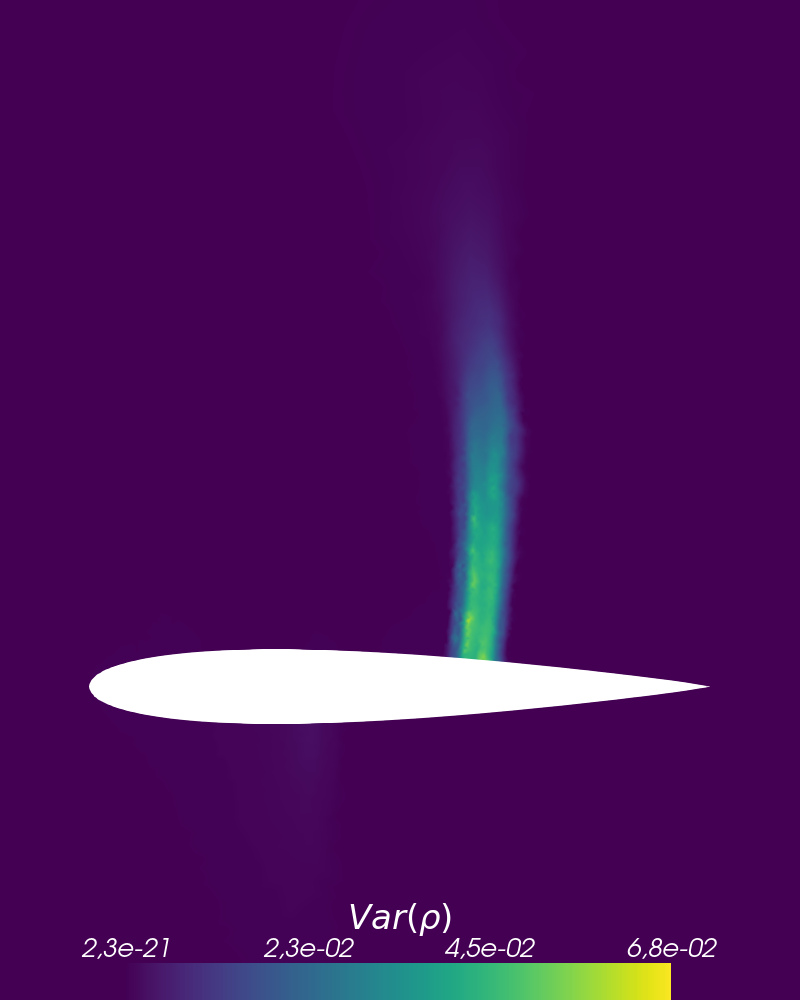
\includegraphics[scale=0.2]{figs/Euler1DPlots5/sg_4_9_VarRho.png}
		\label{fig:sub2}
	\end{subfigure}%
	\hfill
	\begin{subfigure}{0.3\linewidth}
		\centering
		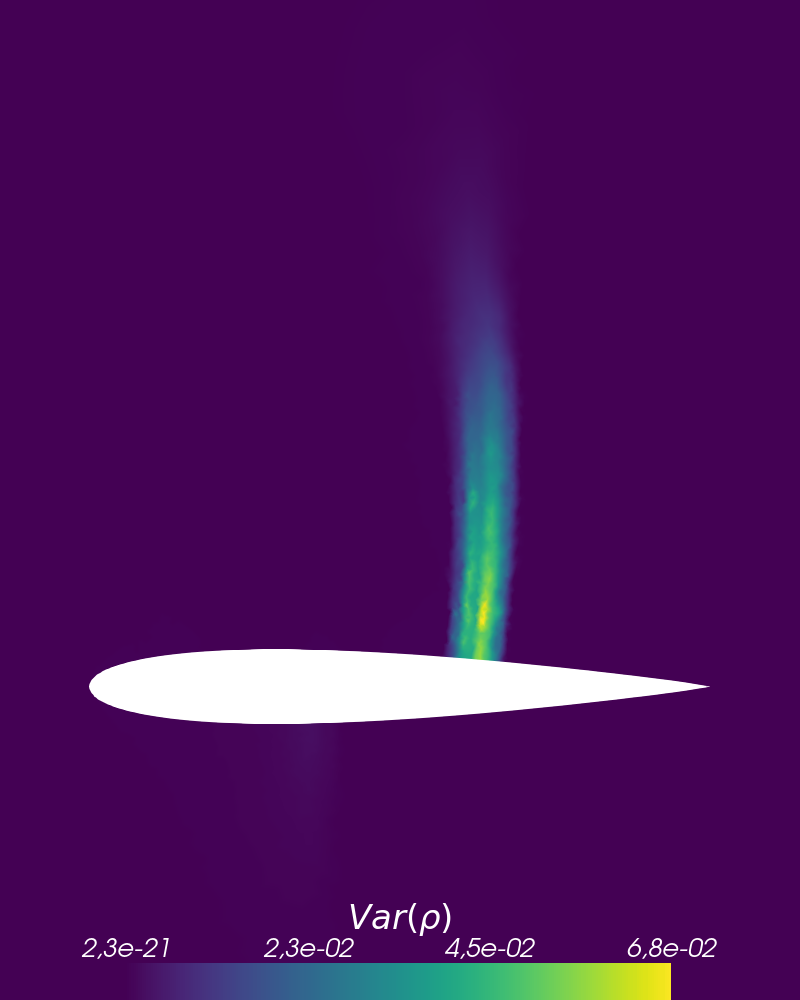
\includegraphics[scale=0.2]{figs/Euler1DPlots5/osIPM4-4_VarRho.png}
		\label{fig:sub1}
	\end{subfigure}
	\caption{E$[\rho]$ and Var$[\rho]$ computed with SC$^5$, SG$_4$, IPM$_4$ (from left to right). Compare to the refernce solution shown in Figure \ref{fig:referenceSolution}.}
	\label{fig:ERhoVarRho5}
\end{figure}

Recall that the numerical flux \eqref{eq:numericalFluxIPM} uses a quadrature rule to approximate integrals. We start by investigating the effects this quadrature has on the solution accuracy. For this, we run the IPM method with a moment order ranging from 3 to 7 using a Clenshaw-Curtis quadrature rule with level three (i.e. 9 quadrature points) and level four (i.e. 17 quadrature points). A comparison of the error obtained with these two quadrature levels is given in Figure~\ref{fig:ErrorDifferentQuad}. To denote the quadrature level, we use a superscript and the moment order is denoted by a subscript. We observe the following:
\begin{itemize}
\item When for example comparing the error obtained with IPM$_8^3$ and IPM$_8^4$ (the subscript indicates the polynomial order, the superscript indicates \comment{the number of quadrature points}) it can be seen that the error stagnates when the chosen quadrature is not sufficiently accurate. Hence, the aliasing effects that result from an inaccurate quadrature rule in the numerical flux and not the truncation error of the moment system dominate the accuracy level.
\item If the truncation order is sufficiently small, both quadrature levels yield the same accuracy. Note that this holds for the expectation value until a truncation order of $N=5$ and for the variance for $N=4$. Hence, the variance is more sensitive to aliasing errors.
\item Figure~\ref{fig:ErrorDifferentQuadA} reveals that the IPM error of E[$\rho$] with 9 quadrature points (level 3) stagnates at the error level of SC$^9$, i.e. the aliasing error heavily affects the accuracy. This behavior becomes more dominant when looking at the variance error in Figure~\ref{fig:ErrorDifferentQuadB}. Here, IPM$_8^4$ yields a significantly improved result compared to IPM$_8^3$. Again, the IPM$_8^3$ result stagnates at the SC$^9$ accuracy level, which can be reached with IPM when only using four moments (combined with a sufficiently accurate quadrature level). Hence, the number of moments needed for IPM to obtain a certain variance error is significantly smaller than the number of quadrature points needed for SC. This result can be observed throughout the results of this work. Especially for high dimensional problems, this potentially decreases the number of unknowns to reach a certain accuracy level significantly. However note, that since the numerical flux evaluation requires $O(N\cdot Q)$ operations, the numerical costs will depend on the chosen quadrature rule.
\end{itemize}
Let us now compare stochastic-Collocation with stochastic-Galerkin and IPM as well as its proposed acceleration techniques at a fixed moment order 9. Note that since IPM generalizes SG, all proposed techniques can be used for stochastic-Galerkin as well. Stochastic-Collocation uses quadrature levels $2,3$ and $4$, which corresponds to $5,9$ and $17$ quadrature points. All adaptive methods use gPC polynomials of order 2 to 9 (i.e. 3 to 10 moments). Order 2 uses a level 2, orders 3 to 6 use a level 3 and orders 8 and 9 use a level 4 quadrature rule. When the smoothness indicator \eqref{eq:errorIndicator} lies below $\delta_{-} = 2\cdot 10^{-4}$, the adaptive methods decrease the truncation order, if it lies above $\delta_{+} = 2\cdot 10^{-5}$ the truncation order is increased. The remaining methods have been computed with a level 4 quadrature rule. 

All intrusive methods are iterated until the expectation value of the density fulfills the stopping criterion \eqref{eq:residualSteady} with $\varepsilon = 5\cdot 10^{-6}$, however it can be seen that the error saturates already at a bigger residual. For every quadrature point, SC iterates the solution until the density reaches a certain residual level $\varepsilon$. We observed that the SC error requires a smaller residual level to reach a constant state and we have recorded this behavior in the following Table \ref{tab:resSC17} for the SC$^{17}$ solution. \frama{Sollen wir hier die Ergebnisse zu Frage 1 im zweiten Dokument einbauen?}
\begin{center}
\begin{table}
\resizebox{\columnwidth}{!}{%
\begin{tabular}{ | m{3cm} || m{0.9cm} | m{0.9cm} | m{0.9cm} | m{0.9cm} | m{0.9cm} | m{0.9cm} | m{0.9cm} | m{0.9cm} | m{0.9cm} | m{0.9cm} | } 
	\hline
	residual $\rho$ & 5e-06 & 4e-06 & 3e-06 & 2e-06 & 1e-06 & 9e-07 & 8e-07 & 7e-07 & 6e-07 & 5e-07  \\ 
	\hline
	error E[$\rho$] in e-03 & 1.506 & 1.464 & 1.438 & 1.401 & 1.368 & 1.360 & 1.359 & 1.358 & 1.358 & 1.357  \\ 
	\hline
	error Var[$\rho$] in e-03 & 1.339 & 1.332 & 1.292 & 1.248 & 1.217 & 1.215 & 1.214 & 1.213 & 1.213 & 1.213  \\ 
	\hline
\end{tabular}
}
\caption{Error values at various residual levels when using SC.}
\label{tab:resSC17}
\end{table}

\end{center}
Hence, we can deduce that SC requires a smaller residual to converge to a steady state solution. Therefore, the results for SC$^{17}$ will be presented for a residual of $\varepsilon = 5\cdot 10^{-6}$ as well as a reduced residual of $\varepsilon = 10^{-6}$. Note that in the case of SC, the error cannot be recorded without violating the non-intrusive framework and adding extra costs, which is why we only plot the final error and the corresponding run time.    %One possible reason for this behavior could be that SC is less synchronized, meaning that the solution certain quadrature points 

First, let us mention that the adaptive SG method fails, since it yields negative densities during the iteration. The standard SG method however preserves positivity of mass, energy and pressure. The change of the relative L$^2$-error during the iteration to the steady state has been recorded in Figure~\ref{fig:L2ErrorSolution}. When comparing intrusive methods without acceleration techniques as well as SC, the following properties emerge:
\begin{itemize}
\item Compared to IPM, stochastic-Galerkin comes at a significantly reduced runtime, meaning that the IPM optimization problem requires a significant computational effort.
\item SG$_9$ shows a smaller error compared to IPM$_9$ for the expectation value. For the variance, we see the opposite, i.e. IPM yields a better solution approximation than SG.
\item Again, intrusive methods yield improved solutions compared to SC with the same number of unknowns. Actually, the error obtained with 17 unknowns when using SC is comparable with the error obtained with 10 unknowns when using intrusive methods.
\end{itemize}
The proposed acceleration techniques show the following behavior:
\begin{itemize}
\item The One-Shot IPM (osIPM) method proposed in Section~\ref{sec:OneShotIPM} reduces the runtime while yielding the same error as the classical IPM method.
\item When using adaptivity (see Algorithm~\ref{alg:ad-IPM}) in combination with the One-Shot idea, the method is denoted by \textit{adaptive One-Shot IPM} (adosIPM). This method reaches the steady state IPM solution with a faster runtime than SG.
\item The idea of refinement retardation combined with adosIPM (see Algorithm~\ref{alg:adosIPM}) is denoted by retardation adosIPM (readosIPM), which further decreases runtime. Here, we use two different strategies to increase the accuracy: First, we steadily increase the maximal truncation order when the residual approaches zero. To determine residual values for a given set of truncation orders $2,4,5$ and $8$, we study at which residual level the IPM method reaches a saturated error level for each truncation order. The residual values are then determined to be $6e-05,3e-05,2.2e-5$ and $2e-05$. The second, straight forward strategy converges the solution on a low truncation order of $2$ to a residual of $10^{-5}$ and then switches to a maximal truncation order of $9$. Strategy 1 is depicted in red, Strategy 2 is depicted in green. It can be seen that both approaches reach the IPM$_9$ error for the same run time. Hence, we deduce that a naive choice of the refinement retardation strategy suffices to yield a satisfactory behavior.
\end{itemize}

Let us finally take a look at the expectation value and variance computed with different methods. All results are depicted for a zoomed view around the airfoil. Figure~\ref{fig:ERhoVarRho5} shows the expectation value (first row) and variance (second row) computed with $5$ quadrature points for SC and $5$ moments for SG and IPM. One can observe the following
\begin{itemize}
\item All methods yield non-physical step-like profiles of the expectation value and variance along the airfoil. 
\item The jump position of the intrusive solution profiles capture the exact behavior more accurately.
\end{itemize}
The readosIPM results as well as the corresponding refinement levels are depicted in Figure~\ref{fig:readosIPMEVar}. One observes that the solution no longer shows the previously observed discontinuous profile and yield a satisfactory agreement with the reference solution depicted in Figure~\ref{fig:referenceSolution}. The refinement level shows that away from the airfoil, a refinement level of 0 (i.e. a truncation order of 2) suffices to yield the IPM$_9$ solution. The region with a high variance requires a refinement level of 7 (truncation order 9).
\begin{figure}[h!]
\centering
	\begin{subfigure}{0.3\linewidth}
		\centering
		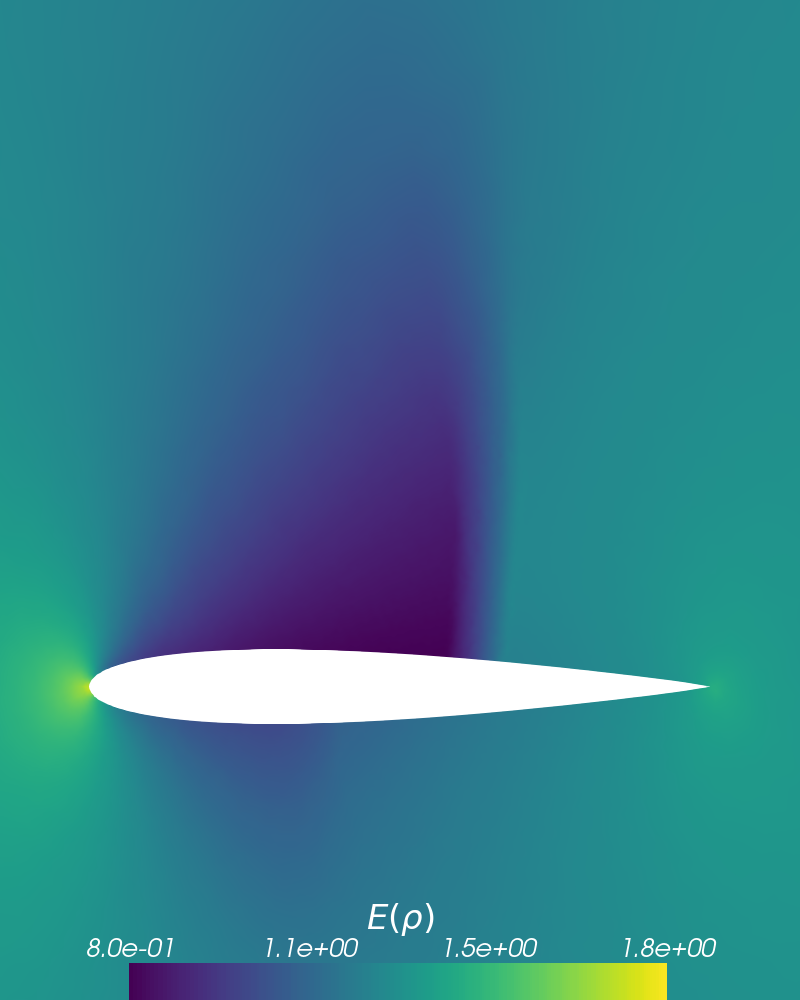
\includegraphics[scale=0.2]{figs/Euler1DPlots10/euler2D_nacaCoarse_refadosipm_n2-9_sg2-4_s05_aoa_oneRet_ERho.png}
		\label{fig:sub1}
	\end{subfigure}%
	\hfill
	\begin{subfigure}{0.3\linewidth}
		\centering
		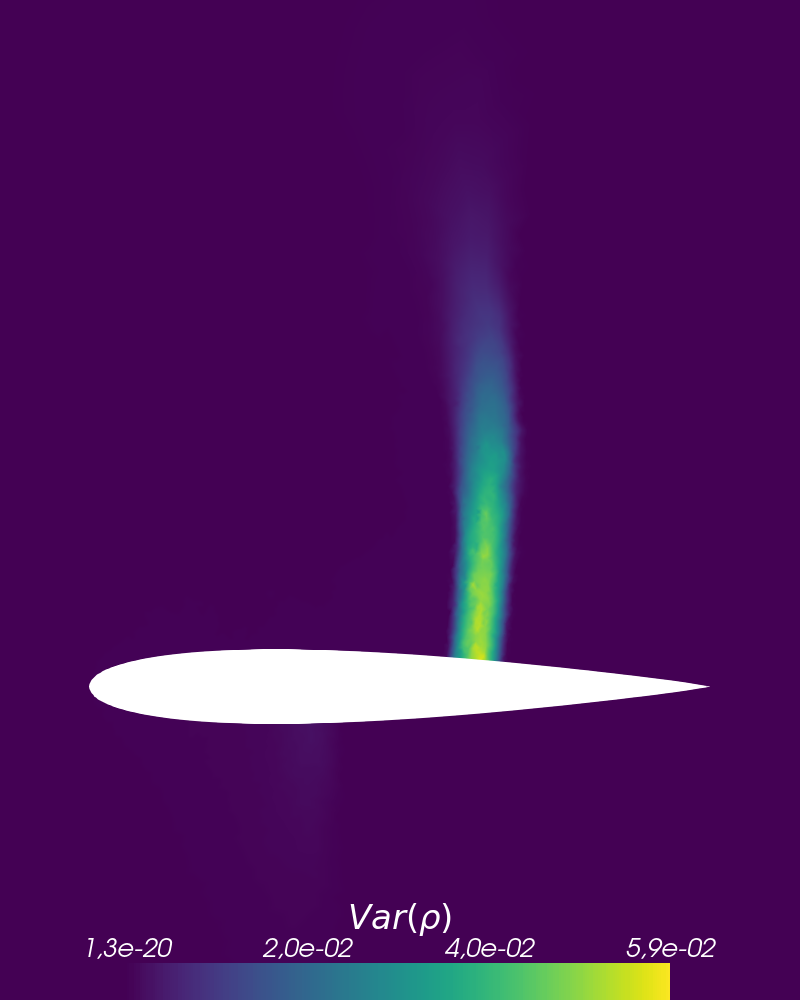
\includegraphics[scale=0.2]{figs/Euler1DPlots10/euler2D_nacaCoarse_refadosipm_n2-9_sg2-4_s05_aoa_oneRet_VarRho.png}
		\label{fig:sub2}
	\end{subfigure}%
	\hfill
	\begin{subfigure}{0.3\linewidth}
		\centering
		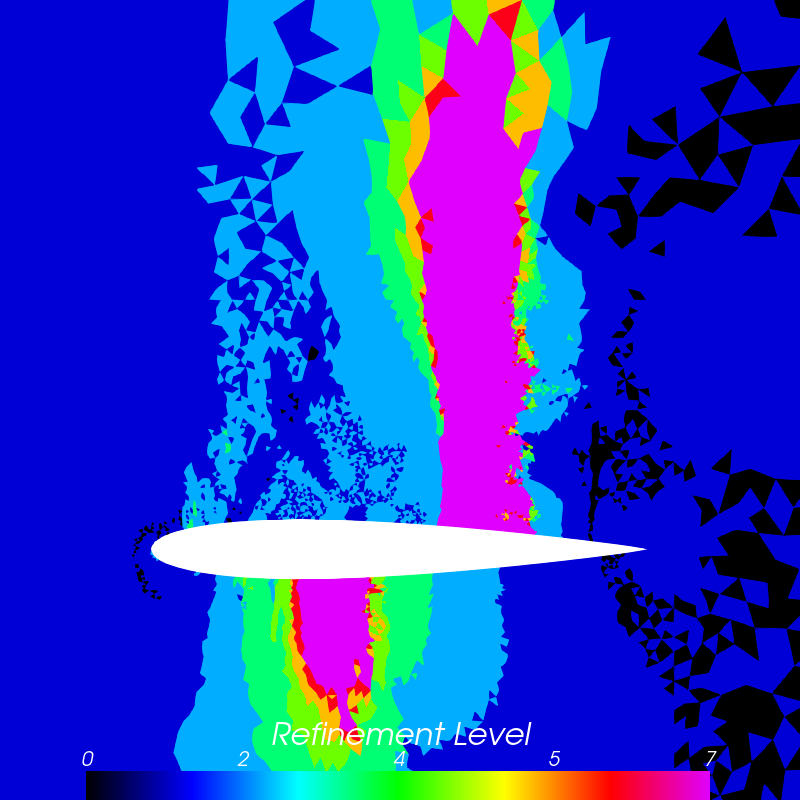
\includegraphics[scale=0.2]{figs/Euler1DPlots10/euler2D_nacaCoarse_refadosipm_n2-9_sg2-4_s05_aoa_oneRet_refinementLevel.png}
		\label{fig:sub1}
	\end{subfigure}
	\caption{E$[\rho]$, Var$[\rho]$ and refinement level for readosIPM$_{2-9}$}
	\label{fig:readosIPMEVar}
\end{figure}

%\begin{figure}[h!]
%\centering
%	\begin{subfigure}{0.33\linewidth}
%		\centering
%				\includegraphics[scale=0.2]{figs/Euler1DPlots10/{EulerSC4-17Res1e-6_errors_ERho}.png}
%		\label{fig:sub1}
%	\end{subfigure}%
%	\begin{subfigure}{0.33\linewidth}
%		\centering
%				\includegraphics[scale=0.2]{figs/Euler1DPlots10/{euler2D_nacaCoarse_sg_n9_sg4_s05_aoa_errors_ERho}.png}
%		\label{fig:sub2}
%	\end{subfigure}%
%		\begin{subfigure}{0.33\linewidth}
%		\centering
%				\includegraphics[scale=0.2]{figs/Euler1DPlots10/{euler2D_nacaCoarse_ipm_n9_sg4_s05_aoa_errors_ERho}.png}
%		\label{fig:sub2}
%	\end{subfigure}
%	\caption{Errors E$[\rho]$ for SC$^{17}$, SG$_{10}$, IPM$_{10}$ (from left to right).}
%	\label{fig:ErrorsERho}
%\end{figure}
%\newgeometry{top=2.5cm, left=2.5cm}

\subsection{2D Euler equations with a two dimensional uncertainty}

In the following, we assume a fixed angle of attack with $\phi = 1.25$ degrees and study the effect of two sources of uncertainties, namely the farfield pressure and Mach number. The farfield pressure is ${p \sim U(100\;325,102\;325)}$ Pa and the Mach number is $Ma \sim U(0.775,0.825)$. Since this problem has only a two-dimensional uncertainty, we use a tensorized quadrature set, which in our experiments proved to be more efficient than a sparse grid quadrature. For SC, we use quadrature sets with $5^2$, $9^2$ and $17^2$ quadrature nodes and compare against SG with moments up to total degree $9$ as well as adaptive IPM with refinement retardation (with and without the One-Shot strategy). The IPM method uses moment orders ranging from $1$ to $9$ adaptively with refinement barriers of $\delta_{-} = 1\cdot 10^{-4}$ and $\delta_{+} = 1\cdot 10^{-5}$. The refinement retardation allows the truncation order to have a maximal total degree of $1$ until a residual of $\varepsilon = 1.5\cdot 10^{-5}$ and then increases the truncation order by one when the residual is reduced by an amount of $5\cdot 10^{-6}$. Hence, the maximal truncation order of $9$ is reached when the residual is below $\varepsilon = 7\cdot 10^{-6}$. Again, the refinement strategy let to negative densities for SG resulting in a failure of the method.
\begin{figure}[h!]
\centering
	\begin{subfigure}{0.5\linewidth}
		\centering
				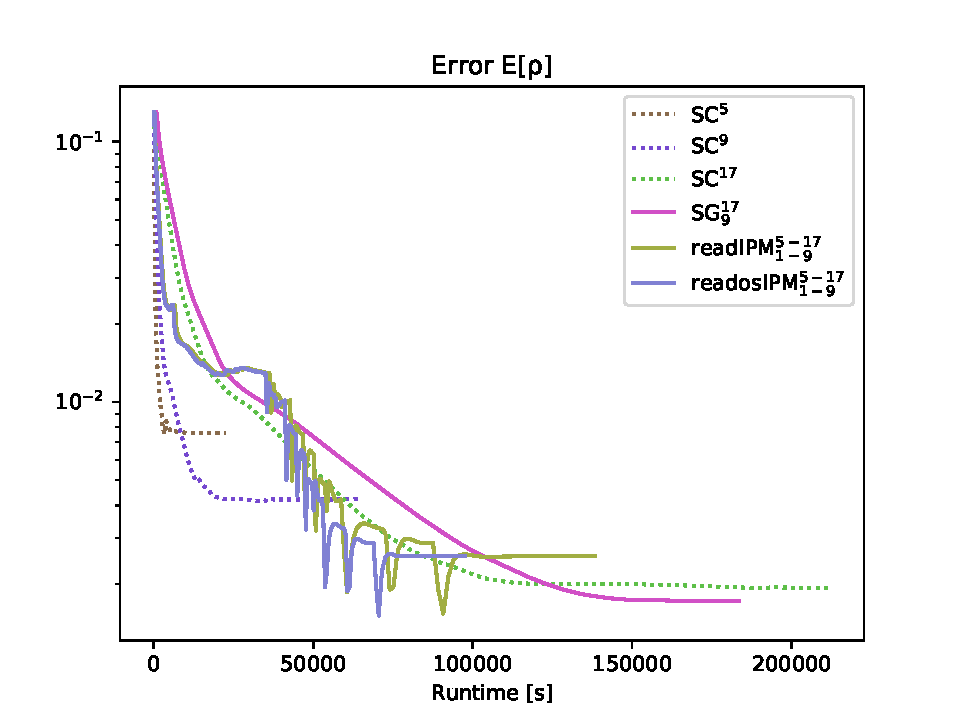
\includegraphics[scale=0.5]{figs/Euler2D/L2_error_E[rho].pdf}
		\label{fig:sub1}
	\end{subfigure}%
	\begin{subfigure}{0.5\linewidth}
		\centering
				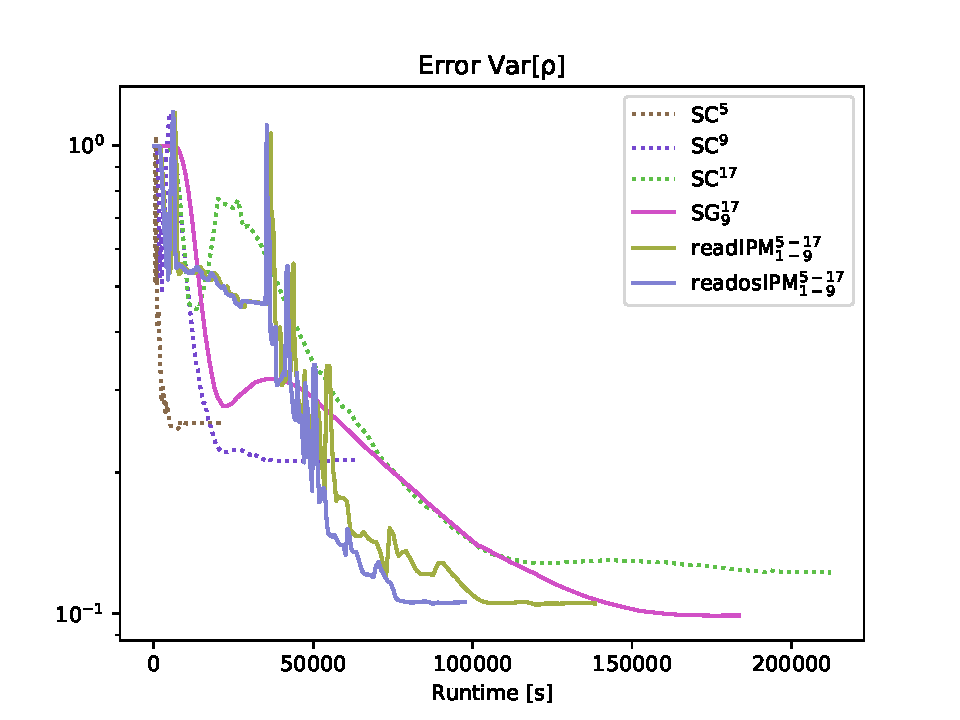
\includegraphics[scale=0.5]{figs/Euler2D/L2_error_Var[rho].pdf}
		\label{fig:sub2}
	\end{subfigure}
	
	\begin{subfigure}{0.5\linewidth}
		\centering
				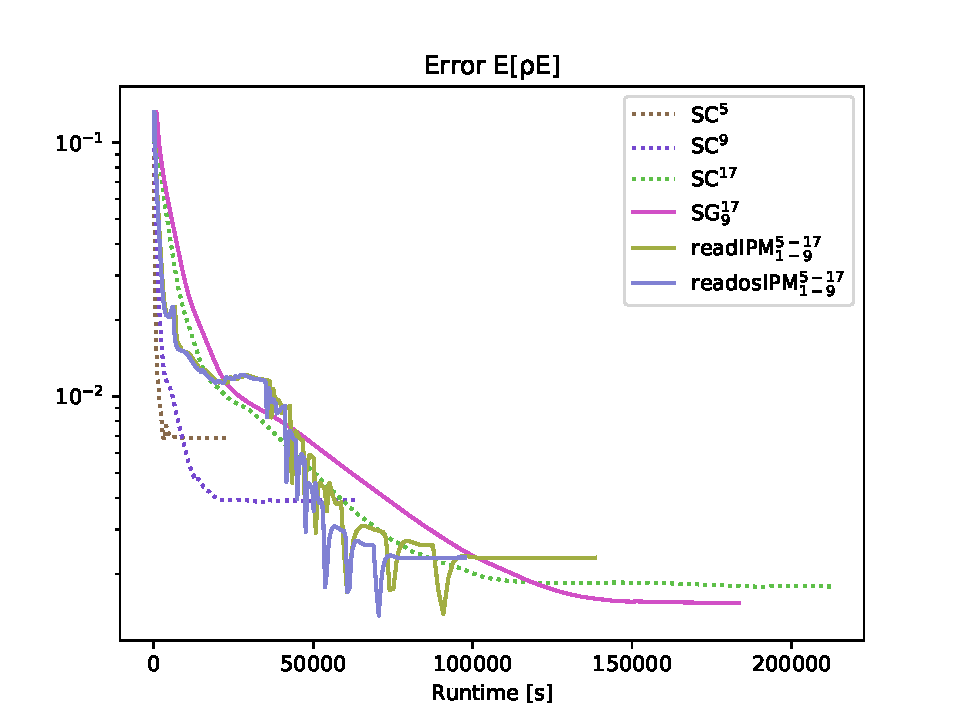
\includegraphics[scale=0.5]{figs/Euler2D/L2_error_E[rhoE].pdf}
		\label{fig:sub1}
	\end{subfigure}%
	\begin{subfigure}{0.5\linewidth}
		\centering
				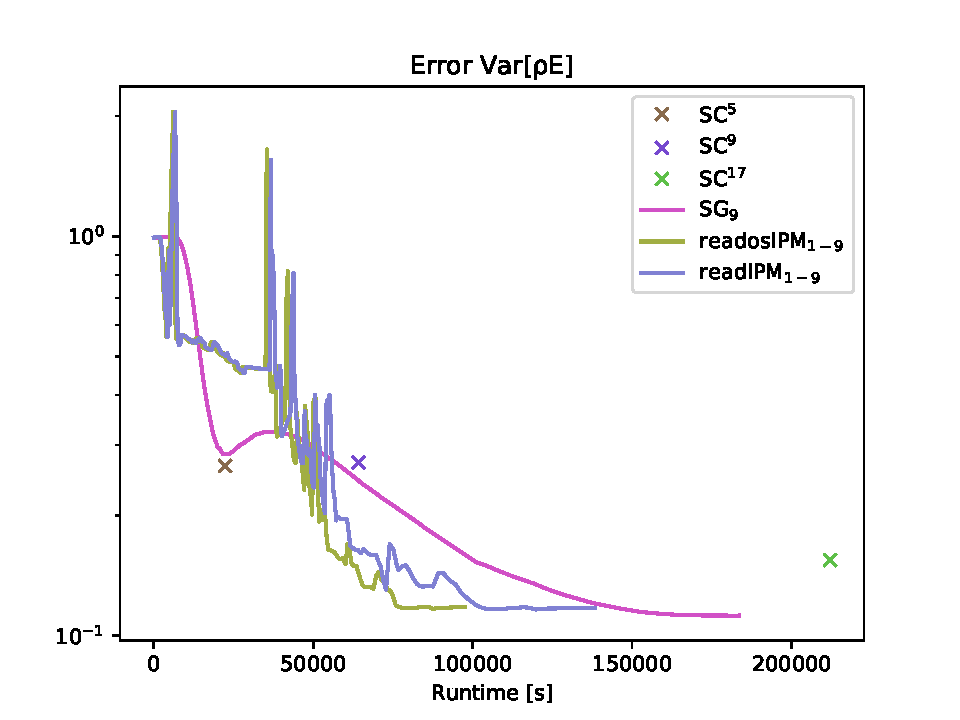
\includegraphics[scale=0.5]{figs/Euler2D/L2_error_Var[rhoE].pdf}
		\label{fig:sub2}
	\end{subfigure}
	\caption{Relative L$^2$-error with 16 MPI threads for density and energy.}
	\label{fig:L2ErrorSolution2D}
\end{figure}
The error during the iteration has been recorded in Figure~\ref{fig:L2ErrorSolution2D}. To determine the error, we used Stochastic-Collocation with a $50$ by $50$ Gauss-Legendre quadrature rule. As in the one-dimensional NACA testcase, the acceleration techniques lead to a heavily reduced runtime of the IPM method. Furthermore, the error obtained with the intrusive methods requires a total degree of $M = 9$, i.e. $N = 55$ moments to reach the error level of SC with 17 quadrature points per dimension i.e. $17^2 = 289$ collocation points. Note that this effect has also been observed in the one-dimensional case, however now for multi-dimensional problems, the reduced number of unknowns needed for intrusive methods to obtain a certain error weighs in more heavily. This shows one promising characteristic of intrusive techniques and points to their applicability for higher dimensional problems. In contrast to before, the SG error level is smaller than the IPM error for both, the expectation value and variance. Furthermore, when comparing IPM with and without One-Shot, one can observe that the effect of this acceleration strategy weighs in more heavily than it did for the one-dimensional case. This behavior is expected, since every iterate of the optimization problem becomes more expensive when the dimension is increased. This means, using a method with less iterations for every computation of the dual variables heavily reduces computational costs, which is why we consider the One-Shot strategy an effective approach, especially for problems with high uncertain dimension.
\begin{figure}[h!]
\centering
	\begin{subfigure}{0.5\linewidth}
		\centering
				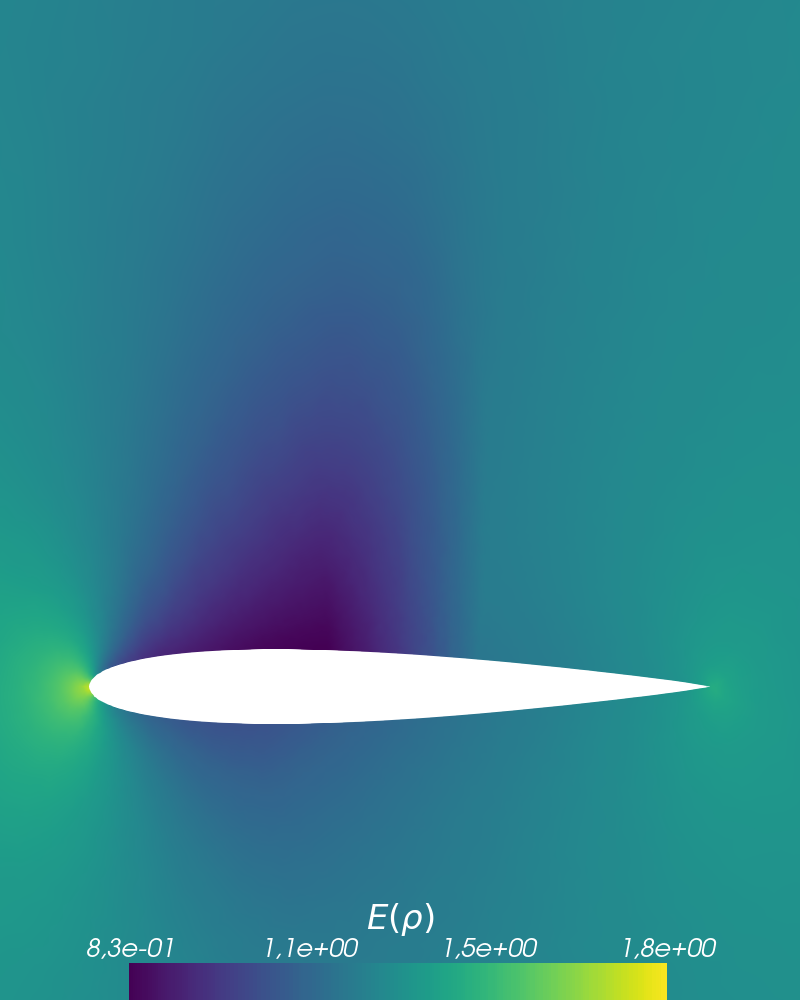
\includegraphics[scale=0.2]{figs/Euler2D/sc50UncertainMaSigma0-025PSigma1000-0Dim2_ERho.png}
		\label{fig:referenceSolutionsub1}
	\end{subfigure}%
	\begin{subfigure}{0.5\linewidth}
		\centering
				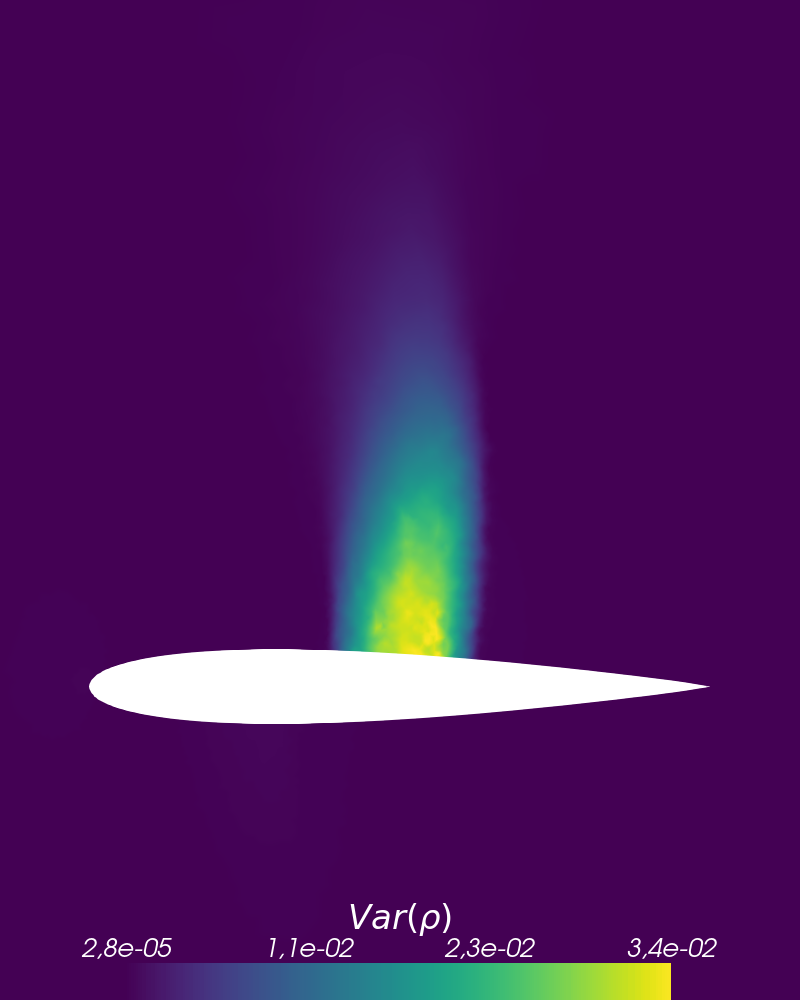
\includegraphics[scale=0.2]{figs/Euler2D/sc50UncertainMaSigma0-025PSigma1000-0Dim2_VarRho.png}
		\label{fig:referenceSolutionsub2}
	\end{subfigure}
	\caption{Reference solution E$[\rho]$ and Var$[\rho]$.}
	\label{fig:referenceSolution2D}
\end{figure}
\begin{figure}[h!]
\centering
	\begin{subfigure}{0.3\linewidth}
		\centering
		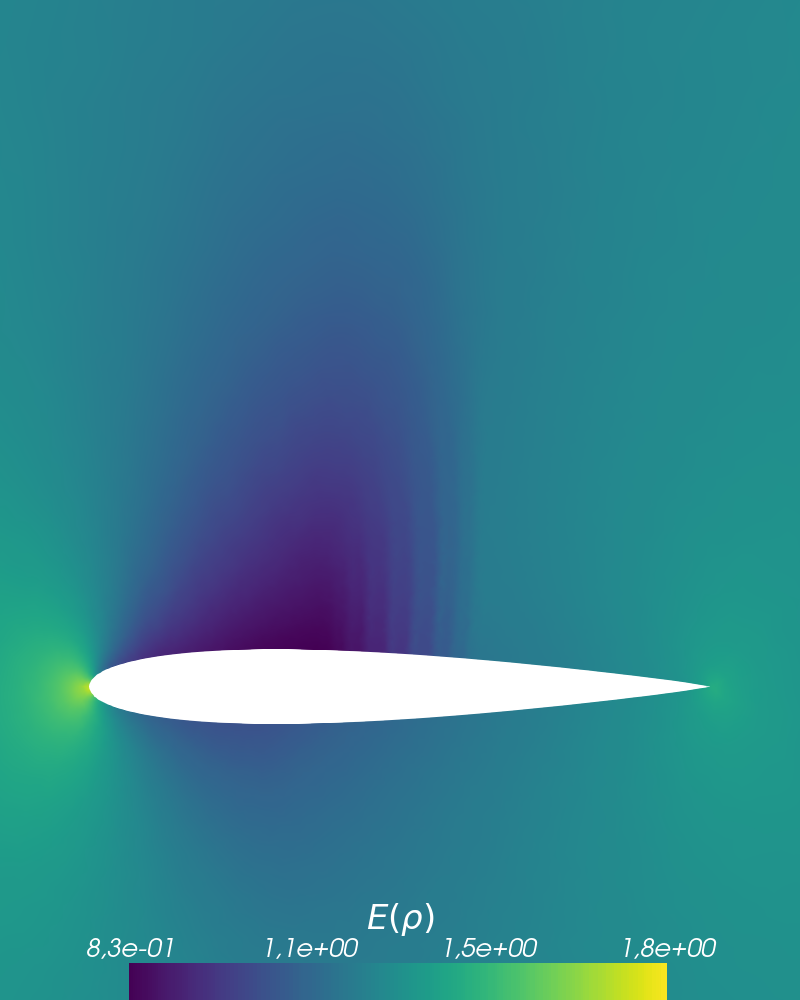
\includegraphics[scale=0.2]{figs/Euler2D/retadosIPM9-4MaP_4_ERho.png}
		\caption{}
		\label{fig:sub1}
	\end{subfigure}%
	\hfill
	\begin{subfigure}{0.3\linewidth}
		\centering
		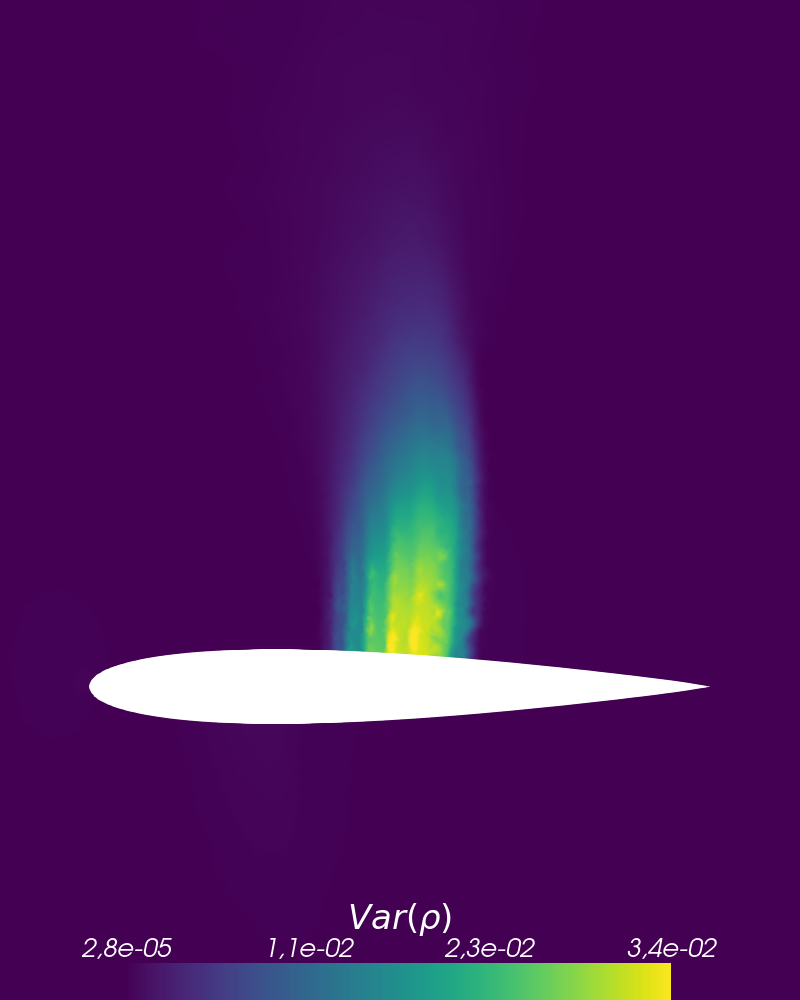
\includegraphics[scale=0.2]{figs/Euler2D/retadosIPM9-4MaP_4_VarRho.png}
		\caption{}
		\label{fig:sub2}
	\end{subfigure}%
	\hfill
	\begin{subfigure}{0.3\linewidth}
		\centering
		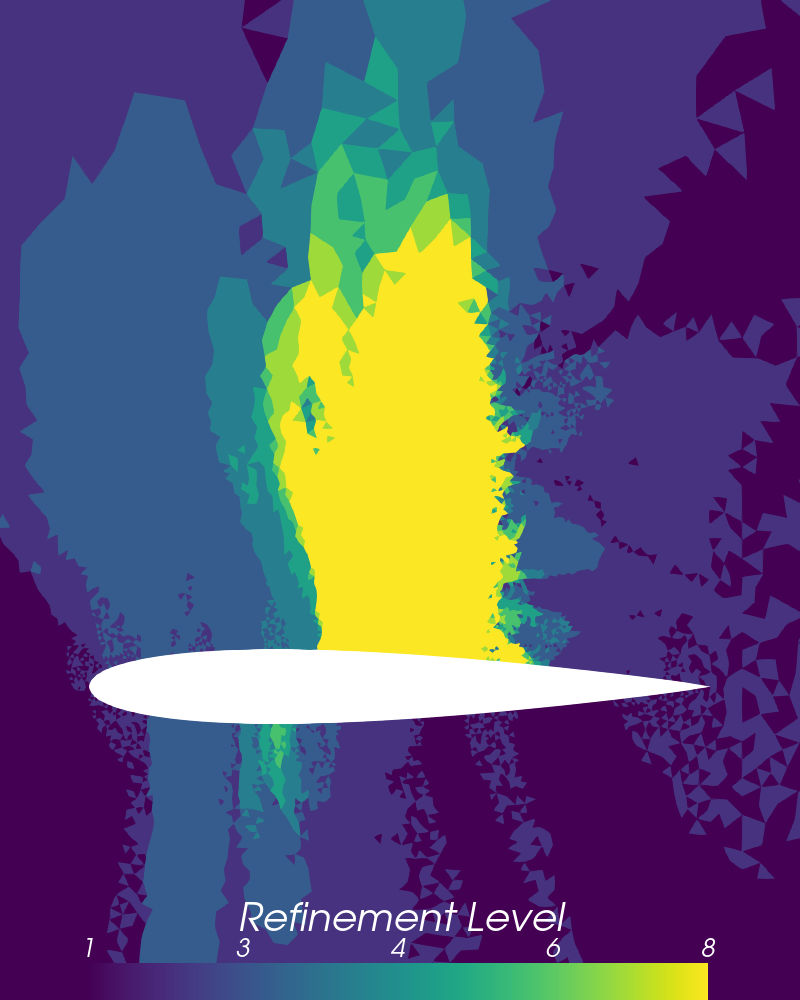
\includegraphics[scale=0.2]{figs/Euler2D/retadosIPM9-4MaP_4_refinementLevel.png}
		\caption{}
		\label{fig:readosIPMEVar2DRefinement}
	\end{subfigure}
	\caption{(a) E$[\rho]$, (b) Var$[\rho]$ and (c) refinement level for readosIPM$_{1-9}$}
	\label{fig:readosIPMEVar2D}
\end{figure}
When looking at the computed IPM expectation value and variance in Figure~\ref{fig:readosIPMEVar2D} and compare the results against the reference solution in Figure~\ref{fig:referenceSolution2D}, one can observe that since the uncertainty effects the result more heavily than in the one-dimensional case, the IPM solution still shows a step-like profile. However, we are able to capture the main features of the reference solution. The increased effect of the uncertainty can again be seen in Figure~\ref{fig:readosIPMEVar2DRefinement}, where a refinement level of $8$, i.e. a truncation order of $9$ is chosen on a larger portion than for the one-dimensional case.

\subsection{Pipe Testcase}
\begin{figure}[H]
	\centering
	\begin{subfigure}{0.5\linewidth}
		\centering
		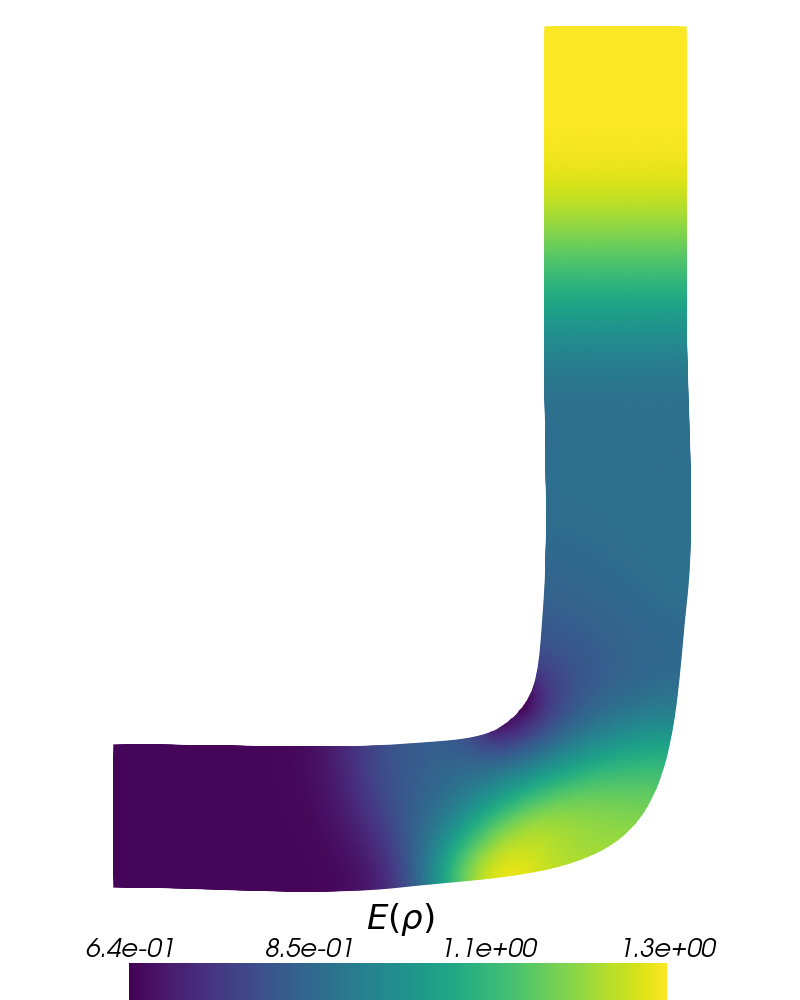
\includegraphics[scale=0.2]{figs/pipe/pipe_sc_ref_n50_E(rho).png}
		\label{fig:referenceSolutionsPipe1}
	\end{subfigure}%
	\begin{subfigure}{0.5\linewidth}
		\centering
		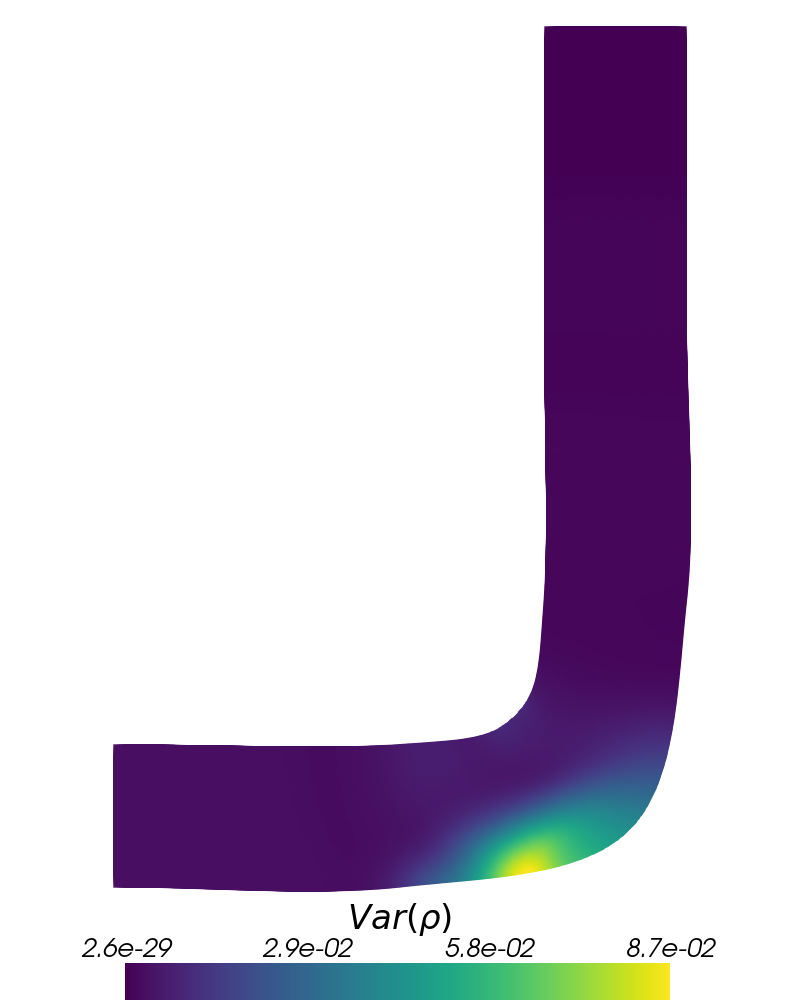
\includegraphics[scale=0.2]{figs/pipe/pipe_sc_ref_n50_Var(rho).png}
		\label{fig:referenceSolutionsPipe2}
	\end{subfigure}
	\caption{Reference solution E$[\rho]$ and Var$[\rho]$.}
	\label{fig:referenceSolution3D}
\end{figure}
\comment{TODO: Pipe testcase}